\newcommand*{\ra}{Recursive Alignment}%
\subsection{\ra{}}
\begin{figure}
	\centering
	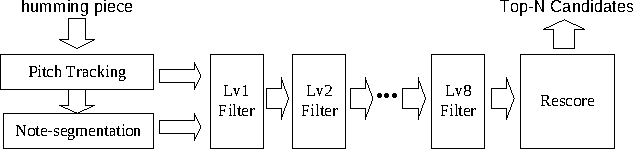
\includegraphics{wu2006top}
	\caption{Block διάγραμμα από \protect\cite{wu2006top}. Πρώτη χρήση RA σε σύστημα QbSH.}
	\label{fig:wu2006top}
\end{figure}
\forceendwrapfig{}
Η έννοια του αλγορίθμου \ra{} για matching σε συστήματα QbSH εμφανίστηκε πρώτη φορά το 2006 στο \cite{wu2006top}.
Ο RA διαφέρει από τον αλγόριθμο δυναμικού προγραμματισμού \hyperref[sub:DTW]{DTW},
ο οποίος δουλεύει με frame-to-frame λογική και μπορεί να "χάσει" την γενική εικόνα.
Είναι αλγόριθμος που δουλεύει με top-down λογική.
Δηλαδή, προσπαθεί να ταιριάξει το σχήμα του query και του target ολικά και μετά πραγματοποιεί τοπικές αλλαγές.
Σε κάθε αναδρομική του κλήση, ο αρχικός αλγόριθμος RA, καλεί τον \hyperref[sub:ls]{Linear Scaling} αλγόριθμο,
χωρίζοντας κάθε φορά το query $Q$ και το υποψήφιο note sequence για match $N$.

Σύμφωνα με το \cite{wu2006top},
ο RA είχε τότε καλύτερα αποτελέσματα σε σχέση με τον Linear Scaling και, σε μικρότερο βαθμό, τον DTW ενώ είχε παρόμοιους χρόνους εκτέλεσης.
Ωστόσο, αυτή η υπεροχή του RA δεν επιβεβαιώνεται πάντα σε λοιπές έρευνες.
Το block διάγραμμα του προτεινόμενου συστήματος QbSH φαίνεται στο \imageref{wu2006top}.

Πέρα από την αρχική δημοσίευση ο αλγόριθμος RA χρησιμοποιήθηκε σε επόμενες έρευνες όπως:
\begin{itemize}
\item Στο \cite{ryynanen2008query} χρησιμοποιείται στην υλοποίηση στο MATLAB.
\item Στο \cite{wang2012query}, που φαίνεται στο \imageref{wang2012query}, σαν ranking algorithm πριν την επιστροφή των αποτελεσμάτων.
\item Στο \cite{guo2012query}, που φαίνεται στο \imageref{guo2012query}, σαν ranking algorithm πριν την επιστροφή των αποτελεσμάτων σε συνδυασμό με τα αποτελέσματα από την μετρική Scaling Factor.
\item Στο \cite{guo2013query}, που φαίνεται στο \imageref{guo2013query}, προτείνεται ένας νέος αλγόριθμος key transposition recursive alignment (KTRA).
Ο KTRA προσπαθεί να λύσει το πρόβλημα της διαφοράς στα μουσικά κλειδιά για διαφορετικούς χρήστες (πχ διαφορά ανάμεσα σε άντρες και γυναίκες).
Προτείνει την ολική μετατόπιση του query sequence για την βελτιστοποίηση της απόστασης RA.
\end{itemize}

\undef{\ra}
